This chapter describes the process of desigining the molecule chip experiment.
This was motivated by three main factors: the need to integrate with the
existing experiment, the core proposal of confining molecules close to a
microwave guide, and the practicalities of fabricating the chip.

Each of these factors will be addressed in order. We begin with a discussion of
the existing experiment, and where the chip fits into it. We will see that this
lead us to the conclusion that magnetic traps would be most suitable for our
experiment. Trapping close to the microwave guides requires brining the
molecules close to the surface of the trap, a loading procedure that was
thorourghly investigated with simulations, and analysis of the phase-space
acceptance of the traps. Problems arising from fabrication will mainly be
discussed in the following chapter.

\section{Experiment overview}

Our ultracold molecules are created using the methods described above. Our
apparatues, including the proposed chip chamber, are shown in
\myfigref{design:fig:vacuumsystem}. A buffer-gas source is used to create
\CaF{} molecules in the source chamber, with the beam being longitudinally and
transversely slowed before it is captured in a MOT inside the collisions
chamber.

\begin{figure}[htb]
  \centering
  \includegraphics[width=0.7\textwidth]{figs/experiment_placeholder.png}
  \caption{
    \cm{To be replaced with a proper CAD drawing of the experiment}
    A top-down view of the planned \CaF{} experiment is shown. Molecules are
    created in the source chamber in a buffer-gas cell. They are then
    laser-slowed by the methods described in~\cite{} and undergo transverse
    cooling, before being captured in the collisions chamber.
    Here we can cool the
    molecules by the methods described in \cm{thoery ch} and perform
    experiments in collisions as detailed in \cm{cite}. The magnetic transport
    trap (MTT) can transfer a cloud of molecules to the neighbouring tweezer
    chamber (for the optical tweezer experiment). The chip chamber will be
    positioned next to the tweezer chamber, and will receive molecules from the
    MTT in the same way. Inset, an exploded view of the flange assembly. The
    chip is mounted on a PCB for current (and later microwave) delivery. This
    is positioned above a large copper U-wire for intermediary trapping of
    molecules. The U-wire is electrically isolated by alumininium nitride
    plates.}
  \label{design:fig:vacuumsystem}
\end{figure}

The \CaF{} MOT is the powerhouse of our experiment. Captured molecules can be
cooled further (as discussed above) and used as a source for experiments into
collisions with \Rb{} atoms (see \cm{papers}) and optical tweezers. The tweezer
experiment is undertaken in the neighbouring tweezer chamber, which is loaded
by transporting molecules in a magnetic transport trap (MTT), a quadrupole trap
with coils mounted on a transport stage outside the vacuum chamber. This
transport of the molecules is similar to that used in
\inlineref{Lewandowski2003,PhysRevResearch.1.033035} and elsewhere. It will be
discussed further below and in \cm{transport chapter}.

The chip experiment will integrate into this setup as shown in
\myfigref{design:fig:vacuumsystem}. An additional chamber will be mounted
further downstream of the transport stage, so that molecules can be brought
straight through the tweezer chamber from the collisions chamber. The chip trap
will be held here mounted to a flange using the assembly shown in the inset of
\myfigref{design:fig:vacuumsystem} and in
\mysubfigref{design:fig:chipexperiment}{a}.
away from the transport axis. The flange assembly consists of current
feedthroughs and a PCB to deliver trapping currents to the chip, a large copper
heatsink, and microwave feedthroughs. It will be mounted so that the chip
faces the floor, allowing us to trap and then drop the molecules for imaging.

\begin{figure}[ht]
  \centering
  \begin{subfigure}[b]{0.45\textwidth}
    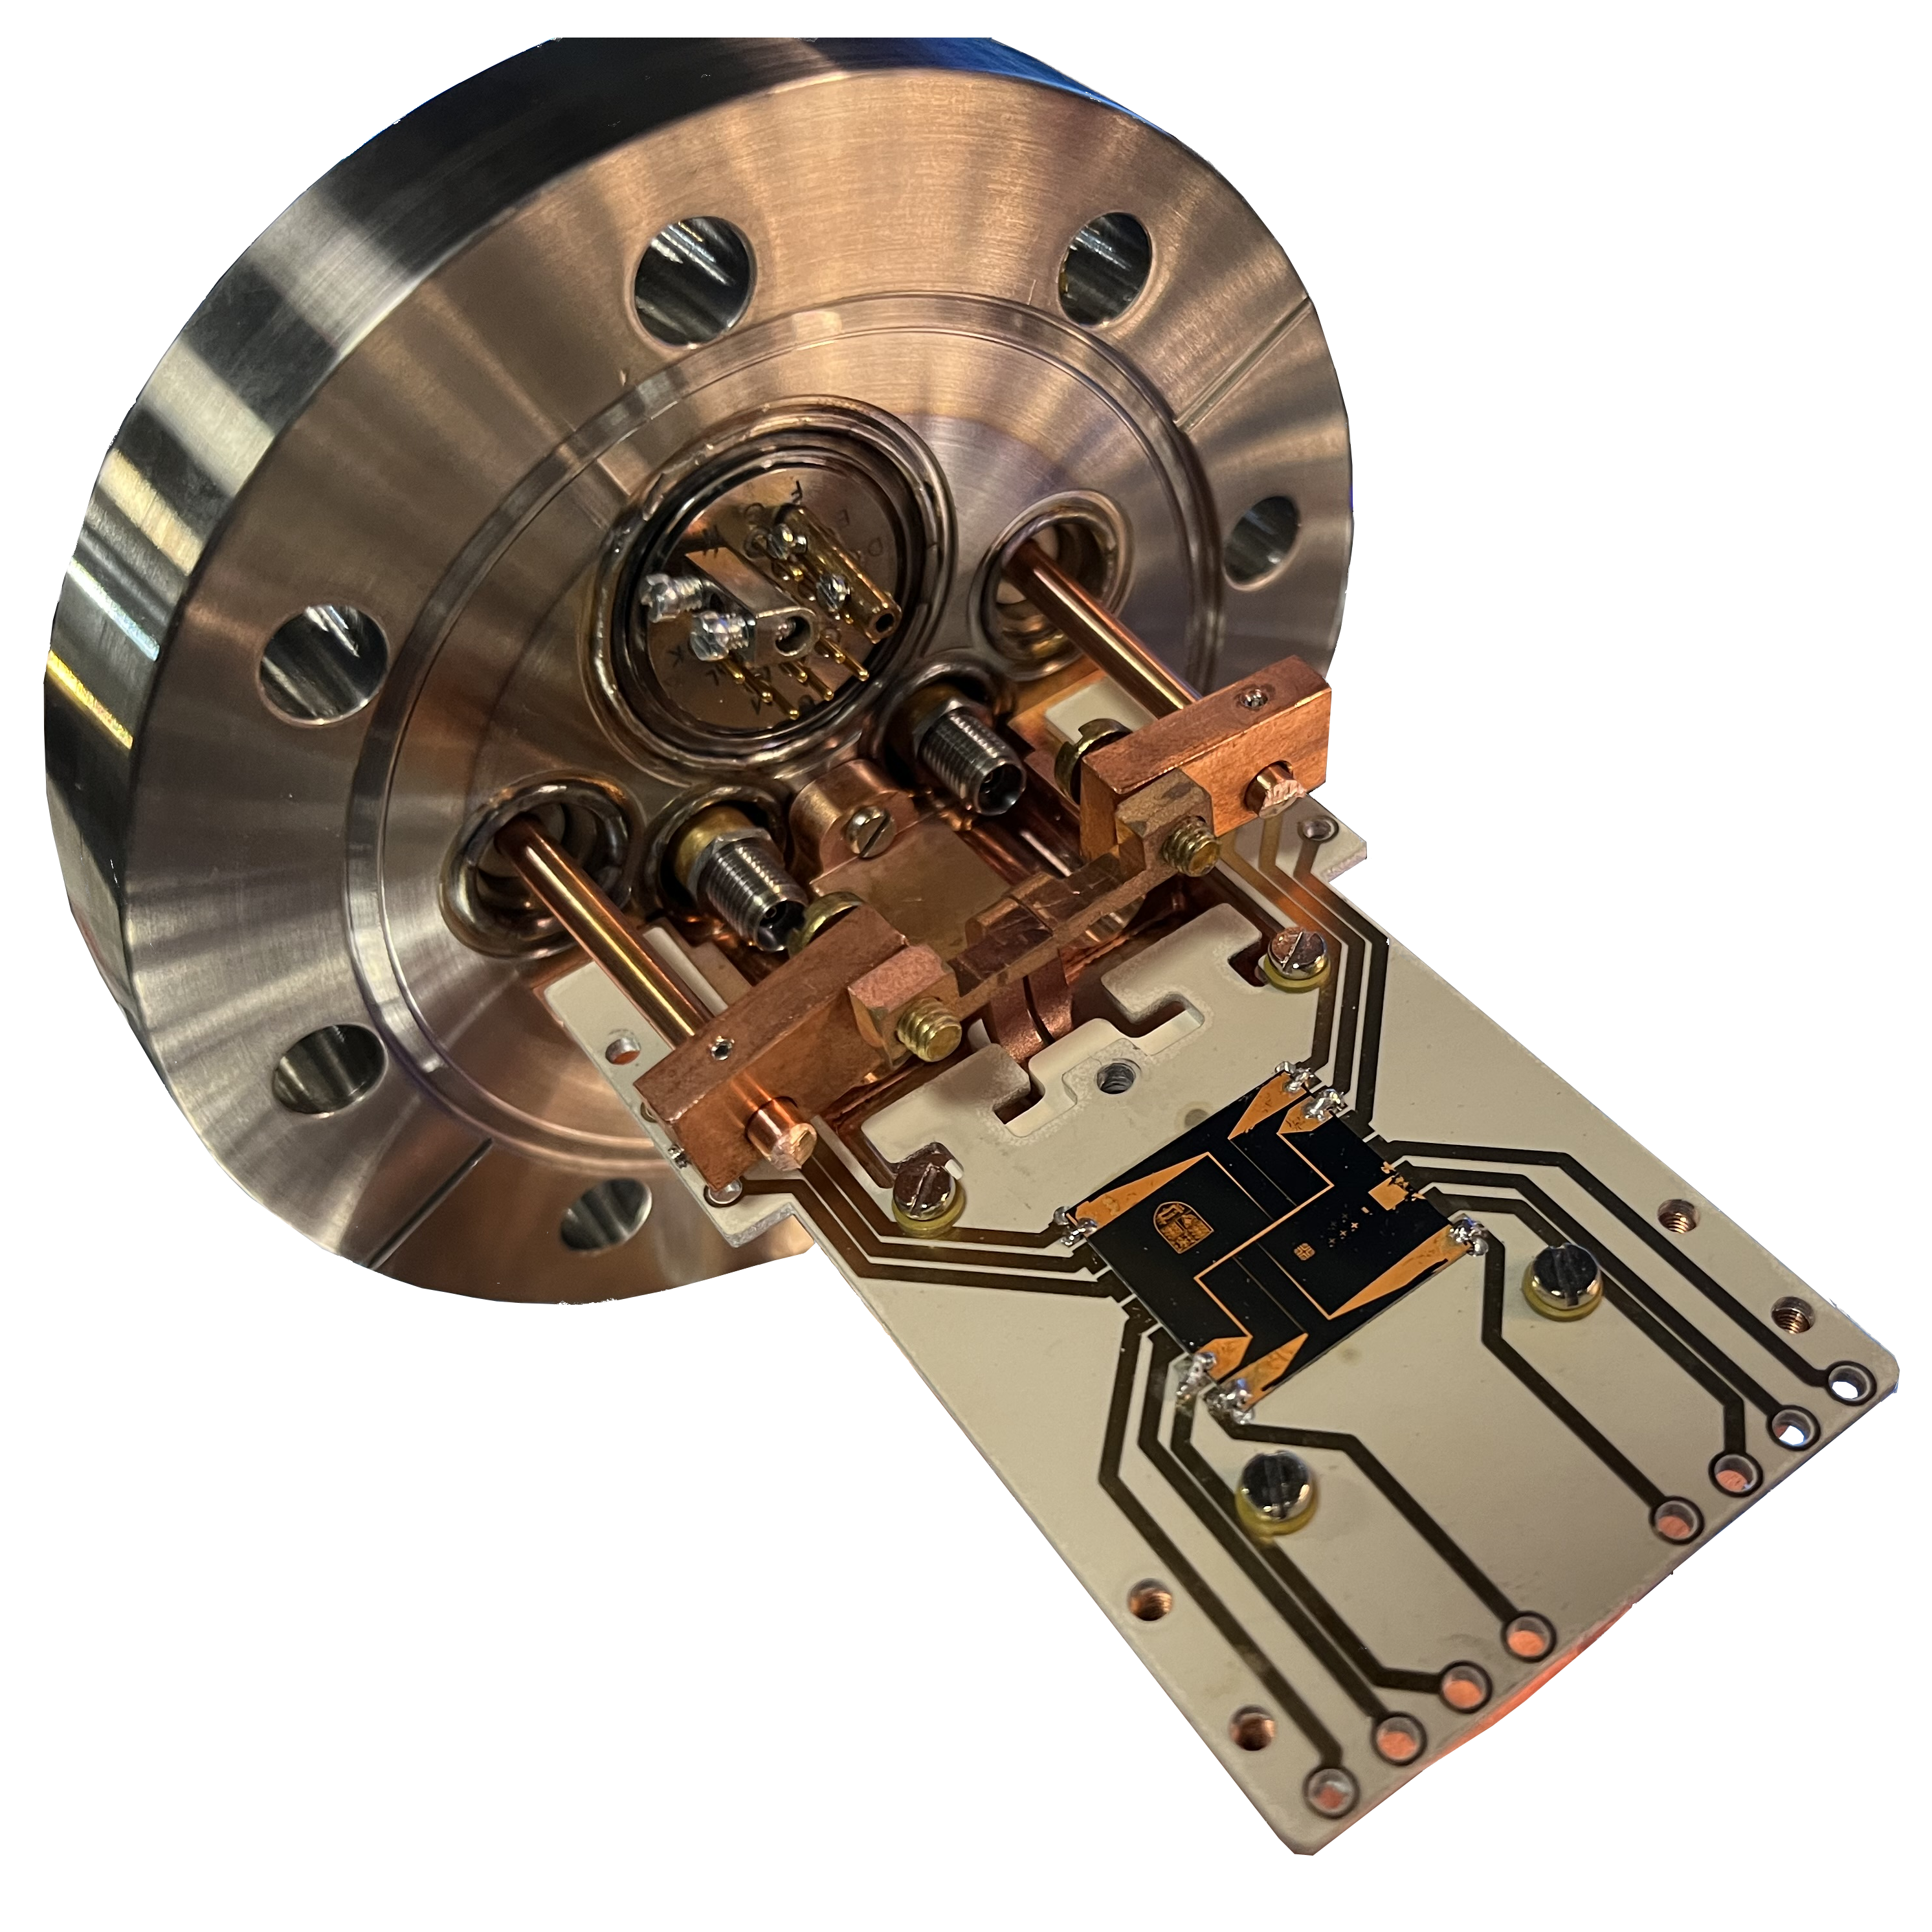
\includegraphics[width=\textwidth]{figs/chip_pic_crop.png}
    \caption{}
  \end{subfigure}
  \hspace{1cm}
  \begin{subfigure}[b]{0.45\textwidth}
    \centering
    \includegraphics[width=\textwidth]{figs/chip_present2.pdf}
    \caption{}
  \end{subfigure}
  \caption{
    In (a) we have the chip assembly fully constructed, with a view of the
    aluminium-core PCB (subchip) for current delivery. Note also the polyimide
    bushings to electrically isolate the retaining screws from the surface. The
    microwave feedthrougs remain disconnected. In (b) we show a schematic of
    the chip features, with the scaling exaggerated for visibility. The three
    overlapping Z-wires are shown. Toward the left is the electroplating
    connection pad and various features used for characterisation, andn the small
  wire there are several anchors to improve adhesion. All of these will be
  discuseed further in chapter~\ref{fab}. The crest of Imperial College London
is also included.}
  \label{design:fig:chipexperiment}
\end{figure}

Since the molecules will be brought into the chamber inside  amagnetic trap,
the natural thing to do seems to be to continue to trap magnetically as we
transfer them onto the chip. Not only does this take advantage of the known,
long-lived \CaF{} states in the trap~\cite{Williams2018}, but it allows us to
follow the well-trodden path of magnetic trapping near a chip, as has been
outlined in previous chapters.  The transfer to the chip will take the
molecules through a series of magnetic traps of decreasing size until they are
in the smallest trap. The design of these traps and the loading
procedure are the main subjects of this chapter.

The first stage of the transfer is a large U wire embedded in the heatsink (see
inset of \myfigref{design:fig:chipexperiment}).  The idea is to use this as a
deep, macroscopic trap that is well-aligned with the chip (by virtue of being
built into the assembly) and can be easily aligned with the MTT, similarly to
other experiments such as \inlineref{Ott2001}.  Since it is under the chip, it
will of course be further from the molecule cloud than the other wires, hence
more current will be required to create a deep trap (as per
equations~\ref{intro:eq:trapbias} and~\ref{intro:eq:trapdepth}). The current is
limited to \SI{100}{\ampere} by the vacuum feedthroughs, allowing for a trap of
depth around \SI{2}{\milli\kelvin} by equation \cm{ref. earlier chapter}.

Once loaded into the U-trap, the molecules will be transferred through the
Z-wire traps on the chip. The idea is that each Z-wire should be sufficiently
large to maintain the currents required to form a trap at height $z$ below the
trap, whilst having a width and height  $w, h \ll z$ so that that the current
is highly localised compared to the cloud size.  This follows the widely-made
assupmption in the literature that the trapping currents are carried by wires
which are infinitesimally small compared to the length scale of the trap
~\cite{2011Ac}.

In the case of the first Z-wire, the molecules are still \SI{4}{\milli\meter}
away from the trapping wire. If we (pessimistically) expect the cloud to have a
temperate on the order of \SI{1}{\milli\kelvin}, then we will require a
trapping current of \SI{30}{\ampere} to form a trap of this depth.  We will
discuss in chapter~\ref{fab} that the maximum wire height achievable is
\SI{5}{\micro\meter}, and we expect that the wires will be able to carry a
maximum current density of \SI{6E10}{\ampere\per\meter\squared}, as was found
for a similar chip design in \inlineref{Treutlein2008}. The Z wire will
therefore have a width $w=\SI{200}{\micro\meter}$. Other wire parameters are
shown in \mytableref{design:table:wires}.

The axial length of the wires also decreases to gradually reduce the size of
the trapped cloud in the $x$ direction. An exaggerated schematic of the wire
layout is shown in \myfigref{design:fig:chipexperiment} and further details are
outlined in \mytableref{design:table:wires}. All wires have been designed to
carry twice the current that is required in the loading scheme.

% TODO Maybe need more detail here
\begin{table}
  \centering
\begin{tabular}{lrrrrr}
  Name & Axis length (\si{\milli\meter}) & Width (\si{\micro\meter})& $I_\text{max}$ & Trap height (\si{\micro\meter}) \\
 \hline
  U & 16 & N/A& 100 & 3000\\
  $\mathrm{Z0}$ & 12 & 200& 60& $3000\rightarrow1000$ \\
  $\mathrm{Z1}$ &  6 & 20& 6& $1000\rightarrow100$ \\
  $\mathrm{Z2}$ &  2 & 2& 0.6& $100\rightarrow10$ \\
 \hline
\end{tabular}
  \caption{Details on the wire dimensions, maximum current, and desired
  trapping heights. The wire design is shown in
  \mysubfigref{design:fig:chipexperiment}{c}. Note that the U wire current is
  limited by vacuum feedthroughs and not by the maximum current calculated by
  the wire dimensions.  The maximum currents have been designed for use at only
  50\% of their potential maximum ($I_\text{max}$).
  }
  \label{design:table:wires}
\end{table}

Each Z trap will begin trapping at one height before the bias field is
increased to bring the trap centre closer to the surface (as per
\myeqref{intro:eq:trapbias}).  To distinguish between the two trap stages for
each wire, we label them $\mathrm{ZX_i}$ for the initial (higher) trap and
$\mathrm{ZX_f}$ for the final (lower) trap, with $\mathrm{ZX}$ corresponding to
the wire labels in \mytableref{design:table:wires}.

A future goal of the project is to incorporate microwave guides onto the chip. This can be
accomplished by adding an insulating layer on top of the wires, on to which we
can fabricate coplanar waveguides~\cite{1127105}. The flange has been designed
with microwave feedthroughs, so that microwaves can be launched onto the
subchip and carried to the chip via coplanar waveguides \cm{to be discussed in
a later chapter}.

Having broadly outlined the experiment, the rest of this chapter will justify
the design of the trapping wires by means of simulation and analysis
of the trapping potentials.

\section{Motion of molecules in a trap}
\label{design:motion}

% TODO Is the Bohr magneton introduced above?
% TODO Do I introduce this ket notation above?
We can assume that the motion of the molecules in the trap is classical. They
move in the potential $V(t, \mathbf{q}) = \mu B(t, \mathbf{q})$, where
$\mu\approx\mu_B$ is the magnetic dipole moment of the molecule in the
$\ket{1,0,-1}$ state.  The motion of any one particle is described by Hamilton's
equations,~\cite{Lichtenberg1969}
%
\begin{align}
  \label{design:eq:hamilton}
  \dot{\mathbf{q}} =  \frac{\partial H}{\partial \mathbf{p}} &&
  \dot{\mathbf{p}} = -\frac{\partial H}{\partial \mathbf{q}},
\end{align}
%
where $H$ is the classical Hamiltonian of the system
\begin{equation}
  %
  H(t, \mathbf{q}, \mathbf{p}) = \frac{\mathbf{p}^2}{2m} + V(t, \mathbf{q}).
\end{equation}
For now we neglect the time dependence of the potential, so that $V(t,
\mathbf{q}) = V(\mathbf{q})$.

Solving Hamilton's equations tells us the position and momentum of a single
particle. Taken together, these two vectors describe a point in a six
dimensional phase-space of position and momentum. The ensemble of
trapped molecules, each one starting at a different point in phase-space, can
be treated by considering the motion of the molecules at its
boundary, and the six-dimensional phase-space volume that this
boundary encloses~\cite{Hand1998}.

It is helpful for us to write the phase-space volume $V$ in terms of the
spatial volume occupied by the ensemble ($V_\text{space}$) and its temperature.
The length-scale for a monatomic gas of temperature $T$ is the thermal de
Broglie wavelength~\cite{blundell2}
%
\begin{equation}
  \lambda_\text{dB}(T) = \frac{h}{\sqrt{2 \pi m k_B T}}.
\end{equation}
%
Hence the unitless phase-space volume is
%
\begin{equation}
  V = V_\text{space} \lambda_\text{dB}^{-3}(T).
\end{equation}
%
It is also useful to define a unitless phase-space
density~\cite{PhysRevA.52.1423}
%
\begin{equation}
  \rho = \frac{N}{V} = \frac{N \lambda_\text{dB}^3}{V_\text{space}}.
\end{equation}
%
For a given cloud with phase-space density $\rho$, trap with volume
$V_\text{trap}$ and depth $T_\text{depth}$,
the maximum possible number of particles that can be trapped is $\rho
V_\text{trap}/\lambda_\text{dB}^3(T_\text{depth})$.

Furthermore, Liouville's theorem~\cite{Landau1982, Hand1998} states that the
phase-space volume is a conserved quantity, as long as the trapping potential
is consevative. This means that the phase-space density of a trapped molecular
cloud cannot be increased without application of some velocity-dependent
damping, such as an optical molasses~\cite{Metcalf1999}. The impact of this for
the chip is that the phase-space density of the cloud at the point of loading
onto the chip determines the maximum number of molecules that can be trapped in
the final trap.

If we do not introduce any further cooling steps, then the number of molecules
we are able to trap in the final trap will be
%
\begin{equation}
  N_\text{final} = \frac{\rho_\text{\CaF{}}V_\text{trap}}
  {\lambda_\text{trap}^3} = \frac{\rho_\text{\CaF{}} V_\text{trap}(2 \pi m_\text{CaF} k_B
  T_\text{trap})^\frac{3}{2}}{h^3}
  \label{design:eq:psd_N}
\end{equation}
%
where $\rho_\text{\CaF{}} = 3.4\times10^{-12}$ is the phase-space density of
the \CaF{} cloud after cooling in the blue-detuned molasses~\cite{Truppe2017},
$V_\text{trap}\sim(\SI{10}{\micro\meter})^3$ and
$T_\text{trap}=\SI{4}{\kelvin}$. The \CaF{} mass is
$m_\text{\CaF{}}=\SI{9.79E-26}{\kilogram}$. The trap depth used here is for the
smallest trap operating at \SI{3}{\ampere}, and can be calculated using
equation~\ref{intro:eq:trapdepth}. We therefore have
%
\begin{equation}
  N_\text{final} \lesssim 2000
\end{equation}
%
as an upper bound for the number of molecules trapped in the final trap. To
reiterate, this assumes that the entire trap is full, and no excess molecules
have been lost during loading. We will see below that this will not be the
case. A more realistic number of molecules to be trapped can be found by using
two key tools: analysis of the phase-space acceptance of the traps, and direct
trajectory simulation of the cloud.

\subsection{Phase-space acceptance}

\cm{Probably need to cite Hand 1998}

For a particle to be trapped, it is obvious that it must exist within the
spatial region of the trap, and it must not have sufficient energy to escape
from the trap's potential. In other words, the Hamiltonian of the particle
$H(\mathbf{q}, \mathbf{p})$ must be less than the trap depth $T_\text{depth}$.
This relation defines a region of phase-space that we call the
acceptance. Any particles within this region will not have sufficient
energy to escape, and so will remain trapped under classical motion unless
externally influenced (ignoring for example any collisions, decays, Majorana
losses, etc.)~\cite{Lichtenberg1969}.

As an example consdier the one-dimensional case of a harmonic trap found in 
\inlineref{Crompvoets2005}
%
\begin{equation}
  V(z) = \begin{cases}
    0 & |z| > l \\
    -\frac{1}{2}m\omega^2 z^2 & |z| \leq l.
  \end{cases}
\end{equation}
%
Here, any particle which starts with a position $l \leq z \leq l$ will be
trapped, so long as its velocity is not sufficiently large that it will escape
into the $|z|> l$ region. To reach $z=l$ from an initial position $z_0$, the
particle must have kinetic energy of at least
%
\begin{equation}
  \frac{1}{2}mv_0^2 = \frac{1}{2}m\omega^2(l^2 - z_0^2)
\end{equation}
%
where $v_0$ is the initial velocity. It is now clear that a particle is trapped
on the condition that
%
\begin{equation}
  (v_0/\omega)^2 + x_0^2 < l^2
\end{equation}
%
which defines an ellipse in phase-space.

% Note that in the simulation I have omega = 1, so taking omeaga -> 1000 means
% that we end up with the nice circle with v in m/s. The consequence is that
% the simulation ends up lasting 1.2ms rather than 1.2s

This trapping region is can be verified by simulation, as is shown in
\mysubfigref{design:fig:psaeg}{a}, where the trap has been simulated for $m =
1$, $\omega = \SI[parse-numbers=false]{10^3}{\radian\per\second}$ and $l
=\SI{1}{\milli\meter}$. We initialise 2000 particles uniformly distributed with
$|z_0| < \SI{0.2}{\milli\meter}$ and $|v_0|< \SI{1.5}{\meter\per\second}$,
their trajectories are computed for \SI{1.2}{\milli\second} by the methods
described in the next section. The boundary of the acceptance, called the
separatrix is shown in black. All particles that are intialised inside the
acceptance remain trapped and evolve through time in the usual way for a
harmonic potential.  Particles initialised outside the acceptance are rejected
and lost.

It is also instructive to consider anharmonic potentials, for example
%
\begin{equation}
  V(x) = -V_0\cos(\omega z)
\end{equation}
%
which is also presented in \myfigref{design:fig:psaeg}, using the same
parameters as for the previous potential. We again see that particles with
sufficiently low energy in the trapping region remain trapped, however in this
case the anharmonicity of the trap results in the particle cloud spiralling
outwards, undergoing an effective increase in the phase-space density.

Finally, it is useful to consider the phase-space acceptance of a wire trap.
For simplicity we begin by considering only the acceptance in the $z$ direction
(perpendicular to the chip surface). Acceptance of a Z-wire with an axis of
\SI{20}{\milli\meter}, current of \SI{40}{\ampere} and a trapping height of
\SI{3}{\milli\meter}. The particles are initialised such that they have no
motion in the $x$ and $y$ directions, and the trajectories are simulated for
\SI{200}{\milli\second}. The distributions as initialised and at the end of the
simulations are shown in \myfigref{design:fig:psaeg}. The accepted
molecules (blue) are once again those that start inside the sepatrix. There are
also metastable molecules (orange) which remain outside the acceptance but stay
nearby the trap. These are molecules with nearly sufficient energy to escape
the trap, but may take some time to do so.

% TODO This caption
\begin{figure}[htb]
  \centering
  \import{figs/simsThesis/}{psa_1D.pgf}
  \caption{
    The phase-space acceptance for harmonic (a, d), anharmonic (b, e) and
    Z-wire trap (c, e) are shown. The top row shows the initial positions of
    the particles, those that are accepted by the trap are shaded blue,
    particles that are lost are shaded red, and metastable particles in orange.
    The energy contour of the trap depth is also shown. The end state of the
    simulation is shown in the lower row. Note the filamentation effect in (e)
    and (f), where the effective phase-space density of the particles increases
    as they explore regions that are energetically accessible. The harmonic and
    anharmonic examples are inspired by discussion in
    \inlineref{Crompvoets2005}.
  }
  \label{design:fig:psaeg}
\end{figure}

It is therefore clear that a particle that is stored in one trap can be moved
into another if its position in phase space is inside the sepatrix of the new
trap. It is therefore in our interest to design the trapping potentials such
that the emission of one trap overlaps with the acceptance of the next one in
the loading sequence. This is similar to the mode-matching of potentials
described in, for example, \inlineref{2011Ac}. We will see below that the
matching of trap acceptances does indeed allow for reliable loading of the
traps

An adiabatic change to the potential will not affect the phase-space density of
any particles that remain trapped throughout the change~\cite{Hand1998,
Lichtenberg1969}. Hence a cloud of trapped particles can be translated, for
example in the transport coils, or towards the surface of the chip as will be
discussed in section~\ref{design:sim}.

It should be noted that the Liouville theorem also holds for a time-dependent
Hamiltonian. We will see below that the trapping potential will be changed
adiabatically, and make use of the fact that phase-space density is conserved
through this process.

\subsection{Simulating the motion}
\label{design:motion:simmethods}

The motion of a particle can be simulated by numerically solving
\myeqref{design:eq:hamilton}, which we do using Python~\cite{python} and the
symplectic Euler method~\cite{Hairer2015, doi:10.1119/1.2034523} provided by
the Desolver package~\cite{desolver}.  Symplectic methods are powerful tools
for numerically solving Hamiltonian systems whilst conserving energy and
momentum.

We are able to simulate any arbitrary potential, such as those already
discussed in the previous section, but it is useful to consider a more
realistic potential given by the sum of the magnetic and gravitational
potentials,
%
\begin{equation}
  V(t, \mathbf{q}) = V_\text{mag} + mg(z_0-z)
\end{equation}
where $g=\SI{9.8}{\meter\per\second\squared}$ is the acceleration due to
gravity, and $z_0$ is an arbitrary point chosen to be the zero of the
gravitational potential. The actual value chosen does not matter as it
constitutes only a linear shift in the entire potential, we normally present
the potentials with $z_0$ chosen such that the trap minimum is zero.

The Van der Waals attraction between the chip and the molecules is neglected,
since the molecules will (by design) never be close enough to the chip for this
force to be significant.

When simulating the motion of the particles in a quadrupole coil trap (such as
the MTT), the magnetic field is assumed to be an idea quadrupole, so
%
\begin{equation}
  \mathbf{B}(x, y, z) = B'\begin{pmatrix} -x/2 \\ -y/2 \\ z \end{pmatrix}
\end{equation}
where $B'$ is the field gradient.

The magnetic potentials of the wire traps are calculated by considering the
traps to be formed of segments of straight wires, each producing a magnetic
field $\mathbf{B}_\text{seg}^{(i)}$, and the bias field
$\mathbf{B}_\text{bias}(t)$.  The total field is the sum of contributions from
the set of all segments (S), and the bias. The potential is therefore
%
\begin{equation} V\text{mag}(t, \mathbf{q}) = \mu B (t, \mathbf{q}) = \mu
\left| \sum_{i\in S} \mathbf{B}_\text{seg}^{(i)}(t, \mathbf{q}) +
\mathbf{B}_\text{bias}(t)\right|.  \end{equation}
%
Where the field of each wire segment is~\cite{Griffiths2017}
%
\begin{equation} \mathbf{B}_\text{seg}(t, \mathbf{q}) = \frac{\mu_0 I(t)}{4\pi
s_\text{seg}(\mathbf{q})} (\sin(\theta_2)  -
\sin(\theta_1))\hat{\mathbf{\phi}}. \label{design:eq:segmentfield}
\end{equation}
%
Here $s_\text{seg}(\mathbf{q})$ represents the shortest distance between the
point $\mathbf{q}$ and the line that runs through the segment off to infinity
in each direction. We also have the unit vector $\hat{\mathbf{\phi}} =
\mathbf{I}\times\mathbf{q}/(qI)$.

\begin{figure}[h]
\centering
  \begin{tikzpicture}
    % Def coords
    \coordinate (O) at (0, 0);
    \coordinate (L) at (-3, 0);
    \coordinate (R) at (3, 0);
    \coordinate (Q) at (-4, 4);
    % Draw lines
    \draw[line width=0.75mm, ->] (L) -- (R);
    \draw (L) -- (Q);
    \draw (R) -- (Q);
    \draw[<->, densely dotted,shorten >=.5mm,shorten <=.8mm] (Q) -- (-4, 0);
    % Draw line parallel to wire
    \draw[-, dashed] (-5, 0) -- (L);
    \draw[-, dashed] (R) -- (5, 0);
    % Draw dot at Q
    \node at (Q)[circle,fill,inner sep=.5mm]{};
    % Draw angels
    \draw pic[draw,angle radius=1cm,"$\theta_1$" shift={(7mm,2mm)}] {angle=R--L--Q};
    \draw pic[draw,angle radius=1cm,"$\theta_2$" shift={(-7mm,2mm)}] {angle=Q--R--L};
    % Label
    \node[shift={(4mm,0)}] at (Q) {$\mathbf{q}$};
    \node[shift={(2mm, 4mm)}] at (R) {$I$};
    \node[fill=white] at (-5.0, 1.8) {$s_\text{seg}(\mathbf{q})$};
  \end{tikzpicture}
  \caption{Geometry of a wire segment (bold) carrying current $I$, whose field
  can be calculated using \myeqref{design:eq:segmentfield}. The dotted line
  shows $s_\text{seg}(\mathbf{q})$, the shortest distance from the point at
  which the field is calculated ($\mathbf{q}$) to the line parallel with the
  wire (dashed line).
  }
  \label{design:fig:wiresegment}
\end{figure}

In the case of that we are exchanging between
two potentials, the segments of both traps are included in the summation, with
the currents becoming functions of time, and similar for excahnge between a
quadrupole and a wire trap, with the quadrupole gradient being a function of
time.


\subsection{Simulation initialisation}

For all the simulations described below, we begin with a cloud of molecules in
a magnetic quadrupole trap. We use the following initialisation procedure s
that the distribution of our molecules matches that which we expect in the
experiment. 

We begin with a cloud of $N$ molecules whose positions are normally distributed
in all three spatial dimensions with a standard deviation of $\sigma_i$
(typically $\sigma_i = \SI{1}{\milli\meter}$. Similarly the velocity components
are normally distributed with a standard deviation of $\sigma_{v_0}$ (typically
\SI{84}{\milli\meter\per\second}, corresponding to a temperature of
\SI{50}{\micro\kelvin}). 

The cloud is immediately placed in a quadrupole trap with gradient
\SI{10}{\gauss\per\centi\meter}. They are held for \SI{50}{\milli\second}
before the gradient is ramped up over \SI{100}{\milli\second} to the 
\SI{60}{\gauss\per\meter} (the gradient used in the MTT).
The molecules are then held for a further \SI{50}{\milli\second}, as a
stabilisation time.

The increasing trap gradient causes the
molecules to compress as they would when initially loaded into the transport
coils in the MOT chamber, as can be seen in \myfigref{}.
\cm{Need to show histograms in radial and axial, along with comparison to real
data, which I should collect.}

\section{Adiabatic transfer between traps}

% Simple QP ramp (varying time to find adiabatic regime)

In fact, the simple potential of a quadrupole potential can be used to
illustrate a point about transferring molecules between traps. It should be
obvius that if we start with molecules in one potential, then rapidly turn that
one off and turn on another, this will cause heating and increasing its size.
However, if we ramp between the traps adiabatically, then we expect the effect
to the cloud size to be minimal.

In our example, we will consider two ideal quadrupoles with gradients of
\SI{60}{\gauss\per\centi\meter} separated by \SI{3}{\milli\meter} in the $x$
direction. We simulate 2000 \cm{?} molecules using the above-described
initialisation procedure and \cm{sigma and temp values} and ramp between the
potentials in a time $t_\text{ramp}$, which we vary between
\SI{1}{\milli\second} and \SI{100}{\milli\second}. The molecules are then held
for a further \SI{100}{\milli\second}. The state of the system at the end of
the simulation is shown for $t_\text{ramp}\in \{\SI{1}{\milli\second},
\SI{30}{\milli\second}, \SI{100}{\milli\second}\}$ in \cm{figure}, along with
the behaivour of the cloud in the \SI{100}{\milli\second} hold time. Note that
as the ramp time increases, the oscillation in cloud size, temperate and
position decreases, as we have said we expect.

\begin{figure}[p]
\centering
  \import{figs/simsThesis/}{adiabatic_3sim.pgf}
  \caption{
  }
  \label{design:fig:adia3sim}
\end{figure}


The question then is at what point do we enter the adiabatic r\'egime? \cm{Some
figure} shows the cloud width and temperature at the end of the simulation for
varying $t_\text{ramp}$. After $t_\text{ramp}\sim\SI{50}{\milli\second}$ \cm{we
are pretty adiabatic}.

\begin{figure}[tbhp]
\centering
  \import{figs/simsThesis/}{adiabatic_varyramps.pgf}
  \caption{
  }
  \label{design:fig:adiavary}
\end{figure}

\cm{In this figure, note that the rapid oscillations in x width probably
account for the weirdness at the start of the width graph.}

% Z transfer (c.f. rapid)

\section{Trajectory simulation of the initial loading stages}

To ensure that the chip design will allow for robust loading, the loading
process has been simulated up to the $\mathrm{Z0_f}$ trap. This demonstrates
the two main types of transitions in the loading process: handovers between
traps, and compression within a single trap. The timing of the simulation do
not exactly reflect those that will be used in practice, long holding periods
have been inserted between ramps to better illustrate the cause of particle
loss.

The results of the simulation and the parameters of the ramps are outlined in
\myfigref{design:fig:simparams}.
%TODO Redo this old nonsense
\cm{This can be considered in four parts, first
from $t = 0$ to $t=\SI{100}{\milli\second}$ there is a settling period where
the molecules are held in the transport trap. Then there are three
\SI{100}{\milli\second} ramps, each of which is followed by a
\SI{100}{\milli\second} stabilisation period. These three ramps describe the
handover from the transport trap to the U, the U to $\mathrm{Z0_i}$, and the
compression of $\mathrm{Z0_i}$ to $\mathrm{Z0_F}$. They are described in detail
in the following subsections. This simulation used $N=1000$ particles, with one
particle lost during initialisation.}
\cm{For this fig. I think I just want all the parameters, temp, ramps,etc in
one go, similar to before.}



\subsection{MTT - U transfer}
\label{design:sim:trans_U}

\begin{figure}[p]
\centering
  \import{figs/simsThesis/}{mtt_u_summary.pgf}
  \caption{
    The particle distribution in the MTT (blue) and after transfer to the U
    trap (red) following the process described in the main text. The
    phase-space distributions are shown in the $z$-$v_z$ plane in (a) and (b),
    with histograms of the $z$ and $v_z$ projections in (c) and (e)
    respectively. The potentials at the start and end of the transfer are shown
    in (d). Subfigure (f) shows the temperature particle number varying
    throughout the fields are varied in the times that are shaded grey (c.f.
    \myfigref{design:fig:simparams}). \cm{Comment on the results.}
  }
  \label{design:fig:mttusum}
\end{figure}




\cm{Ensure language is consistent when talking about chip, so is the U
above or below?}
%
The first step is to transfer the molecules from the transport coils to the U
wire. This U wire has the largest axial length, and so will be the easiest trap
the transport coils to. The U-wire is also capable of carrying more current
than any of the other wires, which is essential as it is positioned further
from the molecule cloud, beneath the chip.

Between $t=\SI{100}{\milli\second}$ and $t=\SI{200}{\milli\second}$ the current
in the transport coils is adiabtically ramped down while the currents in
the U trap and in the bias coils are ramped up. The molecules are then held
until $t=\SI{300}{\milli\second}$ to ensure that they remain trapped after the
ramp. The simulation parameters are shown in
\mysubfigref{design:fig:simparams}{b}.

The particle loss during the ramp is approximately 10\% of the total. There is
also some heating, which decreases the phase-space density of the cloud. The
cause of this can be seen in \myfigref{design:fig:trans_U}, which shows the
phase-space positions of the molecules at various times throughout the ramp,
and the trapping potential at those times.

\begin{figure}[p]
\centering
  \begin{tabular}{c}
  \import{figs/simsThesis/}{mtt_u_detail_x.pgf} \\
  \import{figs/simsThesis/}{mtt_u_detail_y.pgf} \\
  \import{figs/simsThesis/}{mtt_u_detail_z.pgf}
  \end{tabular}
  \caption{
    Each pair of rows shows the phase-space plots for the MTT to U trap
    handover simulation in the $q_i$-$v_i$ plane, along with the cut-through of
    the potential through the trap centre along $q_i$ at various times. This
    supplements the simulation summary shown in \myfigref{design:fig:mttusum}.
    The superposition of the quadrupole and U-traps briefly causes a lowering
    of the trapping potential, as can be seen at \cm{time??} in the $y$
    direction. Such reductions are not accounted for when considering the
    simple phase-space handovers discussed in the main text.
  }
  \label{design:fig:mttudetail}
\end{figure}

At $t=\SI{175}{\milli\second}$ there is a noticeable decrease in the trapping
depth in the $y$ direction. This is the cause of the particle leak, and occurs
due to the due to the superposition of the two fields causing an overall
decrease in the trap depth in the $x$ and $y$ directions. This only occurs for
a brief period during the ramp (lasting approximately \SI{40}{\milli\second}). 

In addition to the loss during the ramp, we observe a steady loss between
$t=\SI{200}{\milli\second}$ and $t=\SI{300}{\milli\second}$, but only when the
simulation accounts for collision with the chip surface. This loss due to
collision occurs in the U wire because of its position beneath the chip. This
means that the trap is not sufficiently deep to hold our molecules for an
extended period. However the holding time in this simulation is only for
illustration, and the prolonged trapping in the U trap will not be part of the
final experiment. Hence these losses can be ignored.

\subsection{U - Z transfer}
\label{design:sim:U_to_Z0i}

\begin{figure}[p]
\centering
  \import{figs/simsThesis/}{u_z_summary.pgf}
  \caption{
    The U trap to Z trap handover is summarised, with subfigures and colours as
    in \mysubfigref{design:fig:mttusum}. Here we again see loss effects similar
    to those seen for the MTT to U trap handover, with a decrease in trap depth
    \cm{that may be} due to changing from a quadrupole trap to a
    Ioffe-Pritchard trap.
  }
  \label{design:fig:uzsum}
\end{figure}

The U to $\mathrm{Z0_i}$ handover occurs in our simulation from
$t=\SI{300}{\milli\second}$ to $t=\SI{400}{\milli\second}$, shown in
\mysubfigref{design:fig:simparams}{c}.  The phase-space positions of the
molecules and the potentials are shown in \myfigref{design:fig:U_Z0i}.

In the ramp between the transport trap and the U trap, we saw that a hole was
introduced in the trapping potential due to interference between the two
trapping fields. We will see a similar effect when transferring from the U trap
to trap $\mathrm{Z0_i}$.  This time the reduction in depth appears in the $x$
direction, and is due to the current in the U and Z wires opposing each other
on the positive $x$ side. This can be seen in \myfigref{design:fig:U_Z0i} at
$t=\SI{375}{\milli\second}$.

In \myfigref{design:fig:simparams} we see that the loss is again about 10\% of
the particles, however there is no significant change in the phase-space
density. The acceptance of trap $\mathrm{Z0_i}$ is smaller than the emittance
of the U, so this is to be expected.

\subsection{Z compression}
\begin{figure}[p]
\centering
  \import{figs/simsThesis/}{z_summary.pgf}
  \caption{
  }
  \label{design:fig:mttusum}
\end{figure}


In the final stage of the simulation we look at a compression stage. The
trapping potential is adiabatically altered to bring the field minimum closer
to the chip surface. This is achieved by increasing the bias field, but since
this also increases the trap depth the cloud is simultaneously compressed as it
is heated. Since the phase-space density is conserved, the particles heat up in
the trap. This phenomenon is made visible in
\mysubfigref{design:fig:simparams}{d}.

The trajectories and potentials are shown in \myfigref{design:fig:Z0i_Z0f}.
Here the compression in number density and expansion in velocity space is clear
by the changing cloud shape over time. The cloud also clearly follows the
potential minimum without losses.

\begin{figure}[p]
\centering
  \import{figs/simsThesis/}{total_summary.pgf}
  \caption{
  }
  \label{design:fig:mttusum}
\end{figure}


\section{Phase-space acceptance of remaining Z traps}
\label{design:transferbetweenzs}

\cm{Revisit this spiel.}

Once trapped in $\mathrm{Z0_f}$, the remaining loading stages are simply
repeated handovers to the smaller wires, with a compression stage carried out
on each wire to bring the molecules closer to the surface. This is a
well-understood and robust procedure that has been used before to load atom
chips with minimal losses~\cite{Reichel2002}.

That said, since our experiment will operate with a significantly lower phase
space density than previous experiments with atoms, it is important to ensure
that our loading procedure will not suffer from any unnecessary losses. These
compressed traps contain hotter molecules, requiring a smaller time step for
simulation. It is therefore easier to directly examine the acceptance of each
trap.

These are shown in \myfigref{design:fig:phasematchinggrid}, starting with
$\mathrm{Z0_f}$ in row (a). The region of the trap that we expect to be
occupied (as determined by the simulation above) is marked with a dashed line.
This cloud of molecules will be adiabatically transferred into $\mathrm{Z1_i}$.

Since the process is adiabatic, we can anticipate that there will be no
reduction in phase-space density. The cloud of molecules will be transferred to
$\mathrm{Z1_i}$ with negligible heating. However, the total acceptance of the
trap is less than the expected phase-space volume of the cloud, so there
will be particle loss due to spillover.

This was anticipated in section~\ref{design:motion}: phase-space density cannot
increase in a conservative potential, and the acceptance of the smallest trap
will be smaller than the initial cloud in the transport trap. So the final
number of particles will be lower than we started with, as calculated in
\myeqref{design:eq:psd_N}.

Next, $\mathrm{Z1_i}$ is adiabatically compressed to $\mathrm{Z1_f}$, with the
molecules held \SI{100}{\micro\meter} from the surface. Again, this
compression is adiabatic, so we expect no change in the phase-space density.
Compression increases the trap acceptance, so there is also no loss of
particles. This is further supported by the simulated compression of
$\mathrm{Z0_i}$ to $\mathrm{Z0_f}$ discussed above. The acceptance of
$\mathrm{Z1_I}$ is shown in \mysubfigref{design:fig:phasematchinggrid}{b}, with
the expected occupation shown by the dashed line.

Finally, $\mathrm{Z2}$ is loaded and compressed in exactly the same way as
$\mathrm{Z1}$. The adiabatic handover from $\mathrm{Z1_f}$ to $\mathrm{Z2_i}$
is the final cause of particle loss (due to spillover). Then the trap is
compressed to hold the particles \SI{10}{\micro\meter} from the surface, as
shown in \mysubfigref{design:fig:phasematchinggrid}{c}.


\begin{figure}[htb]
\centering
  \begin{overpic}[page=1]{figs/sims/phase_matching_grid.pdf}
    \put(0,68){(a)}
    \put(0,44.5){(b)}
    \put(0,21){(c)}
  \end{overpic}
  \caption{
    A low bound of the acceptance (solid) and expected occupation (dashed) of
    each Z wire trap. This is calculated by finding the acceptance in the weak
    ($x$) trapping direction. Row (a) shows $\mathrm{Z0_f}$, with occupation
    determined by the above simulation. Molecules will be adiabatically
    transferred to $\mathrm{Z1_i}$, which will be fully occupied. Some
    particles will be lost due to the decrease in acceptance but this is to be
    expected, and phase-space density should not increase. In (b) we have the
    acceptance and occupation of $\mathrm{Z1_f}$ following adiabatic
    compression.  Particles will be adiabatically transferred into
    $\mathrm{Z2_i}$, resulting in similar losses to the previous step.  Row (c)
    shows the final acceptance and occupation of $\mathrm{Z2_f}$.
  }
  \label{design:fig:phasematchinggrid}
\end{figure}


\section{Summary}

In this chapter I have presented the design of the chip experiment, starting
with the source of molecules up to the stage of confinement in a Z trap
\SI{10}{\micro\meter} from the chip surface. I have shown that we have created
a loading procedure that will allow us to load this final trap through a series
of wire traps of decreasing size. This is justified by simulation and visual
analysis of the acceptance of the various trapping stages.

The design leaves scope for the addition of microwave guides on a second layer
above the trapping wires, as discussed in chapter~\ref{intro}.
